\documentclass[10pt,a4paper]{article}
\usepackage{rpgcover} % Loads the original rpgmanual.sty and its fonts
\babelprovide[import]{ukrainian}
\usepackage{xsavebox}
\RPGSetRunningTitle{Стежка боргів}
\hypersetup{pdftitle={Стежка боргів — Останній кидок},pdfauthor={Jacopo Biscella}}
\RPGSetCoverWordSpace{.78em}
% IM Fell English and Cinzel Decorative have no Cyrillic: the covers use FreeSerif, as in the adventure.
\renewcommand{\RPGCoverTitleTypeface}{FreeSerif}
\renewcommand{\RPGCoverSubtitleTypeface}{FreeSerif}
\renewcommand{\RPGCoverTextTypeface}{FreeSerif}
\frenchspacing
% Paragraph spacing and leading of the Ukrainian adventure and manual-uk.tex.
\setlength{\parskip}{2.5pt plus .5pt minus .5pt}
\linespread{1.06}\selectfont
% JPEG copies of the shared cover backgrounds (scripts/build-adventure-print-art.sh), as in the adventure.
\RPGSetFrontBackground{assets/engraved-front-background.jpg}\RPGSetBackBackground{assets/engraved-cover-background.jpg}
% The adventure's front-cover typography, with the overlay saved once (xsavebox) and reused on the
% contents page instead of being embedded twice.
\newcommand{\SentieroFrontCover}{%
 \clearpage\RPGCoverPagetrue\thispagestyle{empty}\null
 \xsavebox{SentieroOverlay}{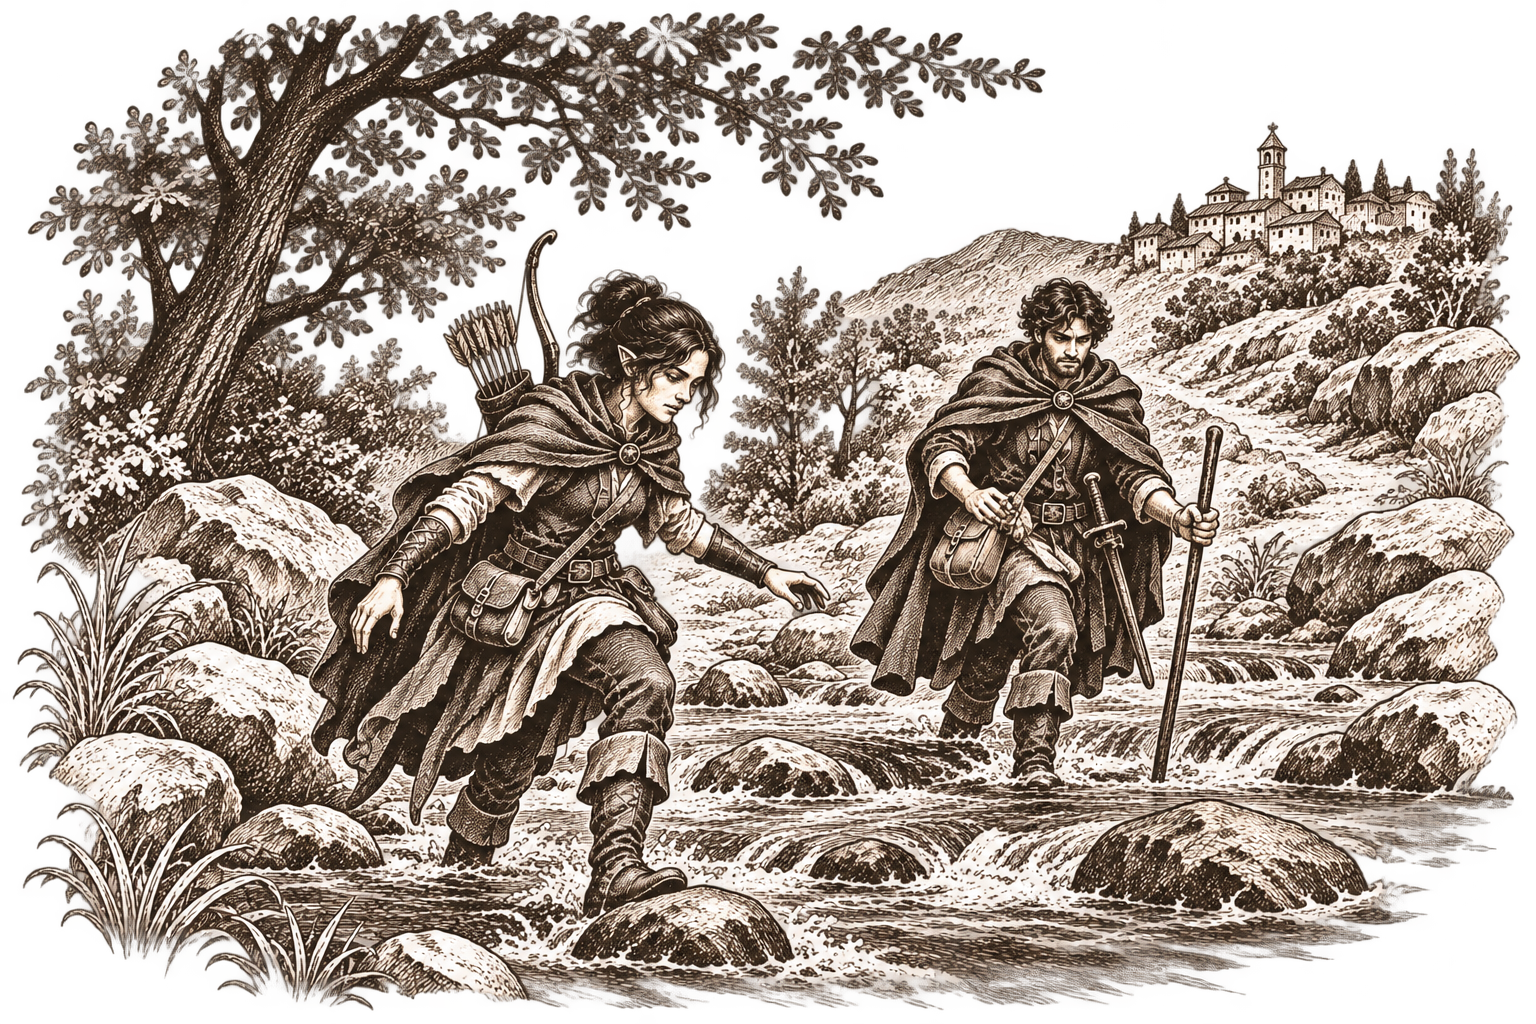
\includegraphics{assets/path-of-debts/front-overlay.png}}%
 \begin{tikzpicture}[remember picture,overlay,x=1mm,y=1mm]
  \RPGDrawBackground{\RPGFrontBackgroundFile}
  % Title and subtitle as on the adventure's cover: same sizes and positions in the cartouche.
  \node[align=center,text=coverink,text width=138mm,inner sep=0pt] at ($(current page.south west)+(105mm,248mm)$)
   {\RPGCoverTitleFont\fontsize{19}{23}\selectfont\spaceskip=\RPGCoverWordSpace\relax СТЕЖКА\\[1.0mm]БОРГІВ};
  \node[align=center,text=coverink,text width=135mm,inner sep=0pt] at ($(current page.south west)+(105mm,235mm)$)
   {\RPGCoverSubtitleFont\fontsize{9.0}{11.6}\selectfont Вступне оповідання для «Останнього кидка»};
  \node[inner sep=0pt,anchor=center] at ($(current page.south west)+(105mm,125mm)$)
   {\resizebox{150mm}{!}{\xusebox{SentieroOverlay}}};
  \node[align=center,text=coverink,text width=124mm,inner sep=0pt] at ($(current page.south west)+(105mm,25mm)$)
   {\RPGCoverTextFont\fontsize{12}{15}\selectfont Jacopo Biscella};
 \end{tikzpicture}
 \clearpage\RPGCoverPagefalse}
% Uses precisely the back background and the editable cover fonts from rpgcover.sty.
% This is text layout only: no substitute illustrations or background graphics.
\newcommand{\SentieroBackCover}{%
 \clearpage\pagenumbering{gobble}\RPGCoverPagetrue\thispagestyle{empty}\null
 \begin{tikzpicture}[remember picture,overlay,x=1mm,y=1mm]
   \RPGDrawBackground{\RPGBackBackgroundFile}
   \node[align=center,text=coverink,text width=170mm,inner sep=0pt]
     at ($(current page.south west)+(105mm,260mm)$)
     {{\RPGCoverTitleFont\fontsize{19}{23}\selectfont\spaceskip=\RPGCoverWordSpace\relax СТЕЖКА БОРГІВ}};
   \draw[coverink,line width=.45pt]
     ($(current page.south west)+(57mm,246mm)$)--($(current page.south west)+(153mm,246mm)$);
   % Blocks at the positions of the adventure's back cover: story at 240 mm, small-caps lines at
   % 197, second rule at 167, description at 162, closing line at 133.
   \node[anchor=north,align=left,text=coverink,text width=137mm,inner sep=0pt]
     at ($(current page.south west)+(105mm,240mm)$)
     {\RPGCoverTextFont\fontsize{10.4}{13.4}\selectfont
      Фальшива монета. Лист без адресата. Двоє подорожніх, які не мали жодної причини довіряти одне одному.\par\smallskip
      Нім Тіслдаун і Мара Вейн ідуть королівським шляхом до Порожнього Вогнища. Дорогою вони дізнаються, що обіцянка може бути небезпечнішою за зброю і що деякі рішення мають наслідки, навіть коли їх ніхто не бачить.};
   \node[anchor=north,align=center,text=coverink,text width=140mm,inner sep=0pt]
     at ($(current page.south west)+(105mm,197mm)$)
     {\RPGCoverSubtitleFont\fontsize{13}{17}\selectfont
      Пролог до пригоди «Дзвін Порожнього Вогнища»};
   \draw[coverink,line width=.45pt]
     ($(current page.south west)+(57mm,167mm)$)--($(current page.south west)+(153mm,167mm)$);
   \node[anchor=north,align=left,text=coverink,text width=137mm,inner sep=0pt]
     at ($(current page.south west)+(105mm,162mm)$)
     {\RPGCoverTextFont\fontsize{10.4}{13.4}\selectfont
      Сім прикладів показують, як рішення гравців перетворюються на кидки, діалоги й наслідки за столом «Останнього кидка».};
   \node[anchor=north,align=center,text=coverink,text width=147mm,inner sep=0pt]
     at ($(current page.south west)+(105mm,133mm)$)
     {\RPGCoverSubtitleFont\fontsize{10.5}{13.2}\selectfont
      Оповідання закінчується там, де починається пригода.};
   \filldraw[fill=white,draw=coverink,line width=.55pt]
     ($(current page.south west)+(139mm,25mm)$) rectangle
     ($(current page.south west)+(187mm,55mm)$);
 \end{tikzpicture}
 \clearpage\RPGCoverPagefalse
}
% Dice icons for the "За столом" boxes, drawn with TikZ (no font glyphs, so they work in every
% language). \Dado{n}: a kept d6 showing n; \Dado*{n}: a rolled die that is not kept (faded).
% \Su and \Giu: the rulebook's keep-highest and keep-lowest arrows, from FreeSerif.
% \Bersaglio: the TN to reach. \Riuscita and \Fallita: success and failure.
\newcommand\DadoPips[1]{%
  \ifcase#1\or \fill (.5,.5) circle (.1);
  \or \fill (.27,.73) circle (.1); \fill (.73,.27) circle (.1);
  \or \fill (.25,.75) circle (.09); \fill (.5,.5) circle (.09); \fill (.75,.25) circle (.09);
  \or \foreach \x/\y in {.27/.27,.27/.73,.73/.27,.73/.73}{\fill (\x,\y) circle (.095);}
  \or \foreach \x/\y in {.25/.25,.25/.75,.75/.25,.75/.75,.5/.5}{\fill (\x,\y) circle (.09);}
  \or \foreach \x/\y in {.28/.22,.28/.5,.28/.78,.72/.22,.72/.5,.72/.78}{\fill (\x,\y) circle (.085);}
  \fi}
\makeatletter
% A die that is set aside has a dashed outline and lighter pips, but stays legible.
\tikzset{dado kept/.style={draw=rpgbrown,fill=white},dado dropped/.style={draw=rpgbrown,fill=rpgshade,dash pattern=on .9pt off .6pt},
  pips kept/.style={fill=rpgink},pips dropped/.style={fill=rpgbrown!70}}
\newcommand\Dado{\@ifstar{\Dado@{dropped}}{\Dado@{kept}}}
\newcommand\Dado@[2]{\tikz[baseline=-.1em,x=.95em,y=.95em]{%
  \path[dado #1,line width=.5pt,rounded corners=1.2pt] (0,-.12) rectangle (1,.88);
  \begin{scope}[shift={(0,-.12)},pips #1]\DadoPips{#2}\end{scope}}}
\makeatother
\newcommand\Su{{\fontspec{FreeSerif}↑}}
\newcommand\Giu{{\fontspec{FreeSerif}↓}}
\newcommand\Riuscita{\tikz[baseline=-.1em,x=1em,y=1em]{\draw[rpgbrown,line width=1.1pt,line cap=round,line join=round] (.08,.35)--(.38,.05)--(.92,.75);}}
\newcommand\Fallita{\tikz[baseline=-.1em,x=1em,y=1em]{\draw[rpgbrown,line width=1.1pt,line cap=round] (.15,.05)--(.85,.75) (.15,.75)--(.85,.05);}}
\newcommand\Bersaglio{\tikz[baseline=-.1em,x=1em,y=1em]{\draw[rpgbrown,line width=.6pt] (.5,.38) circle (.45) (.5,.38) circle (.25); \fill[rpgbrown] (.5,.38) circle (.08);}}
\begin{document}
% Select the language here: babel resets to its main language (english) at \begin{document}.
\selectlanguage{ukrainian}
\RPGStartFrontMatter
\SentieroFrontCover
\RPGStartContents
\clearpage\thispagestyle{rpgfrontmatter}
\vspace*{9mm}
\begin{center}{\fontsize{27}{31}\selectfont\bfseries ЗМІСТ\par}\vspace{9pt}
{\color{rpgline}\rule{.76\linewidth}{.55pt}}\end{center}\vspace{8mm}
\begingroup
\makeatletter
\renewcommand{\l@section}[2]{\@dottedtocline{1}{0em}{4em}{\bfseries #1}{#2}}
\@starttoc{toc}
\makeatother
\endgroup
\vfill
\begin{center}\resizebox{.58\linewidth}{!}{\xusebox{SentieroOverlay}}\end{center}
\vfill
\begin{center}{\small\itshape Вступне оповідання для «Останнього кидка»\par}
\vspace{4pt}{\footnotesize Якопо Бішелла\par}\vspace{5pt}
{\footnotesize Це оповідання, як і «Останній кидок», поширюється за ліцензією Creative Commons Attribution–ShareAlike 4.0 International (CC BY-SA 4.0). Дозволено поширювати й адаптувати його, також комерційно, за умови зазначення автора та збереження ліцензії у похідних творах.\par}\end{center}
\clearpage
\RPGStartMainMatter
\RPGChapter{Лиха монета}
На монеті було дві голови. Одна --- у королівській короні; друга --- з обличчям чоловіка, якого король повісив двадцять років тому.

Учений Мара Вейн покрутив її між великим і вказівним пальцями. Мідь стерлася лише з одного боку. Той, хто її викарбував, хотів, щоб обман протримався недовго: досить, щоб перейти з рук у руки, але замало, щоб потрапити на очі збирачеві податків.

«Я ж казав тобі, що вона фальшива», --- сказав купець.

«Я й не казав, що ні».

«Тоді чого ти вже пів години на неї витріщаєшся?»

«Хочу зрозуміти, хто збирається нею скористатися».

Вони сиділи за столом у поштовому заїзді в Трьох Бродах. Уже четвертий день ішов дощ. Королівський шлях перетворився на довгу смугу багнюки, якою вози й коні просувалися насилу. Купець продав Марі місце на возі, що їхав на північ, а на додачу --- обіцянку: до роздоріжжя Мара зможе переглянути книгу обліку товарів.

Ця обіцянка, як збагнув Мара, була вартіша за саму поїздку.

У книзі були перелічені села, куди їздив віз. Серед них, іншим почерком, було записано \textbf{Порожнє Вогнище}. Біля назви хтось накреслив круглу позначку, а потім закреслив її.

«Того місця вже немає на моєму маршруті», --- сказав купець, помітивши, куди той дивиться.

«Відколи?»

«Відтоді, як ціна на деревину перестала покривати витрати на дорогу».

«А ця позначка?»

Чоловік закрив книгу. «Дрібниця, щоб не забути про доставку. Віз рушає на світанку. Ти ще з нами?»

Мара поклав монету на стіл королем догори. «Так».

Він не сказав купцеві, що багато років тому бачив схожий почерк на берегах старого реєстру. Не спитав і того, чому хтось вишкріб одну дату й вписав іншу. Він давно засвоїв: запитання, поставлені зарано, роблять обережними навіть найнезграбніших брехунів.

Тієї ночі він переписав назву села в кінець своїх нотаток. Потім змінив маршрут. Віз поїде на північ. Мара ж на роздоріжжі зверне на лісову стежку.
\begin{rpgnote}
\textbf{Як читати рамки.} У рамках \emph{За столом} кубики намальовано: \Dado{5}~узятий кубик, \Dado*{2}~відкладений кубик, \Bersaglio~ЦЗ, якого треба досягти, \Riuscita~успіх, \Fallita~невдача. Рівні записано як на аркуші: Недосвідчений 2d6\Giu\ (взяти менший), Компетентний 1d6, Експерт 2d6\Su\ (взяти більший), Винятковий 3d6\Su. ЦЗ — це цільове значення, число, якого треба досягти. Поруч — одна з дистанцій посібника: кілька кроків, можна миттєво дістати.
\end{rpgnote}
\begin{rpgexample}{За столом · Перший кидок}
\textbf{Оповідач:} «Купець закриває книгу. Мара побачив назву села й вишкрібану дату. З першого погляду дату не прочитати. Як ти спробуєш її розібрати?»

\textbf{Гравець Мари:} «Порівнюю сліди цифр з іншими датами, написаними тим самим почерком. Історію я не використовую: мені не треба згадувати, що сталося, мені треба прочитати стерті знаки».

\textbf{Оповідач:} «Тоді це Знання, \Bersaglio\,ЦЗ~4. Мара --- Експерт: кидай 2d6\Su, два кубики, і бери більший».

\textbf{Гравець Мари:} «Кидаю \Dado*{2}\,\Dado{5}: беру 5». \Riuscita

\textbf{Оповідач:} «Успіх. Дата --- два тижні тому, а не вчора. А назву села ти й так уже знав: вона ніколи не залежала від кидка».

\emph{Кидок роблять тоді, коли результат непевний. На рівні Експерт кидають 2d6 і беруть кращий кубик: 5 досягає ЦЗ~4. Ключову підказку ніколи не ховають за кидком.}

\end{rpgexample}
\RPGChapter{Третя дорога}
Нім Тіслдаун не одразу взяла калитку.

Візник тримав її розкритою з виглядом людини, яка чекає на подяку. Усередині лежали шість срібних монет і аркуш паперу, складений учетверо.

«Обумовлена плата», --- сказав він.

«Мабуть, за ту дорогу, про яку знаємо ми обоє».

«За доставку».

«То чому ти сам її не відвезеш?»

Візник показав на свій віз, що стояв зі зламаним колесом біля стайні. «Бо мені бракує коня, колеса й бажання, щоб мене вбили через якогось листа».

Нім розгорнула папір. Він не був запечатаний. На ньому було два рядки: \emph{Половину боргу сплачено. Другу половину --- північним сріблом, коли дзвін замовкне.} Унизу стояла назва заїзду в Порожньому Вогнищі, але не ім’я того, кому лист призначався.

«Хто тобі це дав?»

«Чоловік на роздоріжжі. Сірий плащ, накинутий каптур. Казав правильні слова, але з наголосами не там, де треба, наче вивчив їх на слух».

Нім знову склала аркуш. «А як його звати?»

«Ім’я він не дав. Дав срібло. Береш чи ні?»

Нім узяла калитку, але перелічила монети по одній. Шоста була тонка, майже гладенька. «Двох бракує».

Візник зітхнув і доклав монету. Нім пішла геть, перш ніж він устиг передумати.

Вона не збиралася доставляти листа наосліп. Цих грошей вистачило б на три дні дороги --- забагато за послання без імені. А дзвін, який має замовкнути, --- не та фраза, яку передають, не розуміючи її.

Третя дорога починалася за стайнями, де в багнюці лишилося мало слідів. Швидка стежка, якщо вірити мапі; закинута, якщо вірити місцевим. Нім рушила в путь, рахуючи кроки до першої розвилки.
\RPGChapter{Повалене дерево}
Мара зустрів Нім після полудня, перед стовбуром, що перегородив стежку.

Нім уважно роздивлялася землю. Свою торбу вона поставила на камінь, а в зубах тримала гілочку.

«Ліс зачинено?» --- спитав Мара.

«Залежить від того, як ти любиш скорочувати дорогу».

«Не дуже».

«Тоді в нас є щось спільне».

Буковий стовбур лежав упоперек стежки, корінням досі в землі. Упав він недавно. Листя було зелене, кора --- волога. Такого сильного вітру, щоб його звалити, не було.

Мара присів, щоб роздивитися скалку. Із зарубу сочився прозорий сік.

«Сокира», --- сказав він.

«Дві, --- відповіла Нім. --- Одною рубали з цього боку, другою --- з того».

Мара оглянув зарубки: рівнобіжні, рівні, надто низькі для того, хто прийшов по дрова. «Його зрубали лише для того, щоб перекрити стежку».

«Є сліди, що ведуть назад. А по той бік --- жодних».

«Ти вмієш читати сліди?»

«Я бачу, де їх хтось намагався затерти».

Мара ледь помітно всміхнувся. Нім пролізла під стовбуром, вибралася з рукавом у багнюці й показала на вузьку шпарину між корінням. «Пройти можна, але кому з возом --- тому доведеться повертати».

«А кому з книжками?»

«Залежить, скільки їх».

Мара поплескав по своїй сумці. «Забагато».

Іменами вони обмінялися лише тоді, коли подолали перешкоду. Великим доказом довіри це не було. Але Мара перестав тримати руку на застібці сумки щоразу, як Нім підходила ближче.
\RPGChapter{Зсув}
Зсув вони побачили майже за годину.

Стежка бігла схилом над набряклим струмком. Кроків на двадцять її не стало: дощ відірвав смугу схилу, і на її місці до води сповзав язик багнюки й каміння. Раз у раз якийсь камінь відривався й неквапом котився вниз. Напередодні тут хтось проходив: сліди доходили до половини й зникали під свіжішим зсувом.

Нім оглянула схил. «Можна піднятися назад до броду».

«Скільки на це піде часу?»

«Дві години, а може, й три».

Мара підвів очі. Хмари знову почали затягувати сонце. «А скільки ще до села?»

«Ще пів дня».

«Тоді ми прийдемо вже затемна».

Нім подивилася на зсув. Там, де багнюка оголила скелю, нога могла знайти опору; деінде земля осідала від першого дотику. «Якщо я перейду швидко й легко, схил не встигне зрушити».

«А ще ти можеш упасти».

«Це одна з можливостей».

Мара підтягнув ремінь сумки на грудях. «Тоді сама ти не підеш. Я йтиму за тобою, ставитиму ноги туди, куди ставиш ти, і триматиму тебе за пояс. Якщо послизнешся, я тебе втримаю».

«А якщо послизнешся ти, то потягнеш униз і мене».

«Тоді постарайся, щоб я не послизнувся».

Нім якусь мить дивилася на нього. Потім обернулася до зсуву й рушила. Мара пішов слідом, міцно тримаючись рукою за її пояс.

На півдорозі грудка землі подалася під ногою Нім. Багнюка зрушила вся разом, наче ковдра, яку смикнули за край. Нім хитнуло вперед; Мара вперся п’ятами в камінь і потягнув. Пояс витримав. Якусь мить вони стояли нерухомо, а зрушене каміння котилося вниз до струмка.

Потім Нім намацала ногою скелю, і Мара крок за кроком рушив за нею.

Коли вони дісталися протилежного боку, у Мари тремтіли ноги. Нім обернулася: прохід уже зник під свіжим шаром багнюки.

«Дві години зекономили», --- сказала вона.

«Ти не врахувала десяти років життя, які я щойно втратив».

«Їх на мапі не було».
\begin{rpgexample}{За столом · Перехід і допомога}
\textbf{Оповідач:} «Зсув досі рухається. Щоб перейти його, потрібна Спритність, \Bersaglio\,ЦЗ~4. Якщо провалиш, з’їдеш униз до струмка».

\textbf{Гравчиня Нім:} «У Нім Спритність на рівні Експерт: 2d6\Su. Мара може мені допомогти?»

\textbf{Гравець Мари:} «Я йду просто за нею й тримаю її за пояс. Якщо вона послизнеться, я її втримаю».

\textbf{Оповідач:} «Ви переходите разом, і кидає та, хто йде попереду, --- Нім. У Мари Спритність на рівні Недосвідчений, і Вміння, яке б допомогло, він не має: у цьому ж випробуванні він не кидав би на рівні Експерт, тож його допомога --- некомпетентна. Вона додає кубик до кидка Нім, але ЦЗ зростає з 4 до 5: двоє людей на багнюці зрушують більше каміння. Погоджуєтеся?»

\textbf{Гравчиня Нім:} «Так. Якщо я послизнуся сама, мені не буде за що вхопитися».

\textbf{Оповідач:} «Тоді Нім кидає 3d6\Su\ проти \Bersaglio\,ЦЗ~5».

\textbf{Гравчиня Нім:} «Кидаю \Dado*{1}\,\Dado*{4}\,\Dado{5}: беру 5». \Riuscita

\textbf{Оповідач:} «Ви перейшли. На півдорозі під Нім подається грудка землі, і Мара втримує її за пояс. На тому боці ви обертаєтеся: прохід уже зник під багнюкою. Жоден віз тут не проїде».

\emph{Некомпетентна допомога додає 1d6, але підвищує ЦЗ на 1. З 1, 4 і 5 Нім досягає нового ЦЗ~5. Рука Мари на поясі --- це те, як допомога входить в історію: кидка вона не замінює.}

\end{rpgexample}
\RPGChapter{Двоє на дорозі}
Вони йшли, доки стежка не стала завширшки з дорогу. Тоді й побачили віз.

У воза були високі колеса, кузов, накритий цератою, і сірий кінь, що об’їдав найнижче листя ліщини. Погонич спав на передку, насунувши капелюх на обличчя. Над маточиною правого колеса схилилася жінка.

«Може, допомогти?» --- спитав Мара.

Жінка випросталася. Руки в неї були чорні від мастила, а на поясі висів робочий ніж. «Якщо маєте запасну чеку».

Нім глянула на колесо. «Міняти її не треба. Просто погнувся фіксатор».

«А ти звідки знаєш?»

«Бо чека досі на місці».

Жінка мовчки подала їй молоток. Нім присіла, підважила пласким каменем і завдала трьох точних ударів. Фіксатор випрямився майже до ладу.

«Тепер спробуй», --- сказала вона.

Жінка смикнула колесо. Воно крутилося.

Від стуку погонич прокинувся. Він спитав, хто вони такі, чого лізуть до воза і чи не збираються його пограбувати. Жінка звеліла йому замовкнути.

«Ви їдете до Порожнього Вогнища?» --- спитав Мара.

Жінка перестала витирати руки. «Ще недавно ми там проїжджали».

«А тепер?»

«А тепер краще втратимо день».

Більше вона нічого не захотіла казати, але дала їм шматок хліба й твердий сир, загорнутий у листок. Коли погонич відволікся, вона заговорила впівголоса.

«На північній дорозі повно чоловіків, які збирають мито, хоч не мають на це права. Однострою вони не носять. Один із них колись носив».

«Де?» --- спитала Нім.

«На роздоріжжі Трьох Каменів. Якщо його зустрінете, не кажіть, що допомогли мені».

Мара не наполягав. Перш ніж вони рушили далі, Нім присіла біля колій. Між слідами коня були й інші --- двох пішаків: вони йшли за возом майже до ліщини, а потім повернули назад на північ.

«Це не застереження з чуток, --- сказала Нім жінці. --- Ви їх уже зустрічали».

Жінка глянула на сліди й кивнула. «Один молодий. Другий не показується, якщо може цього уникнути».

Вона відпустила їх кивком і повернулася до воза.
\begin{rpgexample}{За столом · Коли Вміння змінює кидок}
\textbf{Оповідач:} «Фіксатор погнутий. Нім, як ти спробуєш його виправити?»

\textbf{Гравчиня Нім:} «Молотком візнички й каменем як опорою».

\textbf{Оповідач:} «Справжній ремонт --- це Знання з Ремеслами. Але тут треба лише випрямити фіксатор трьома точними ударами: Спритність, \Bersaglio\,ЦЗ~4. Якщо провалиш, можеш його зламати».

\textbf{Гравчиня Нім:} «У Нім Спритність на рівні Експерт: 2d6\Su. Жодне з її Вмінь не стосується молотків, тож додаткового щабля немає. Кидаю \Dado*{3}\,\Dado{5}: беру 5». \Riuscita

\textbf{Оповідач:} «Колесо знову крутиться. Коли ви рушаєте, ти помічаєш сліди біля колій. Хочеш їх роздивитися?»

\textbf{Гравчиня Нім:} «Так. У Нім є Виживання, Вміння Спритності, яке якраз для вистежування».

\textbf{Оповідач:} «Розпізнати, хто йшов за возом, --- \Bersaglio\,ЦЗ~4. Спритність Експерт плюс Виживання: ти піднімаєшся на один щабель, до рівня Винятковий. Кидай 3d6\Su».

\textbf{Гравчиня Нім:} «Кидаю \Dado*{2}\,\Dado*{4}\,\Dado{6}: беру 6». \Riuscita

\textbf{Оповідач:} «Ти розрізняєш два ланцюжки слідів: вони йшли за возом, а потім звернули на північ. Жінка підтверджує, що вже зустрічала фальшивих митників».

\emph{Значення взято з аркуша Нім: Спритність на рівні Експерт, з Виживанням і без Ремесел, які, зрештою, є Вмінням Знання. Доречне Вміння покращує кидок на один щабель. Одна шістка --- ще не Критичний успіх: потрібні щонайменше дві.}

\end{rpgexample}
\RPGChapter{Роздоріжжя Трьох Каменів}
На роздоріжжі було три дорожні камені, але стояли лише два. Третій лежав на боці, наполовину схований у траві. Хтось вирізав у моху свіжий знак: коло, перетнуте рискою.

Нім упізнала знак мандрівного збирача податків. Вона бачила його на розписках, і справжніх, і підроблених, --- підроблених частіше.

«Це мито --- шахрайство», --- сказала вона.

«Не дивина».

«Дивина --- вибір місця. Тут немає нічого, що варто було б охороняти».

«Дорога, --- відповів Мара, --- корисна, навіть коли довкола неї нічого немає».

Запала коротка тиша. Потім із-за кущів пролунав голос.

«Двадцять монет за прохід».

Чоловік, який вийшов на відкрите місце, був молодий. При ньому були завеликий каптан, спис з іржавим вістрям і двоє чобіт від різних пар. Другий чоловік лишився між деревами, там, де стежка знову звужувалася.

«Двадцять? --- перепитала Нім. --- Король, мабуть, став щедрим до своїх збирачів».

«Я не казав, що я від короля».

«Правда. Король принаймні здогадався б послати когось із розпискою».

Юнак опустив спис, націливши його Нім у груди. Мара ступив крок уперед.

«Стривай, --- сказав він юнакові. --- Хто вам наказав тут стояти?»

«Плати або повертай назад».

«Якщо пропустиш нас, --- вів далі Мара, --- не матимеш жодного клопоту. Якщо тебе хтось послав збирати, то, певно, сказав і куди нести гроші».

Юнак завагався. Той, що ховався, кахикнув.

Нім різко обернулася, дивлячись повз них. «На дорозі хтось є».

Молодий митник на мить простежив за її поглядом. Цього вистачило. Нім відвела вістря списа донизу й пройшла повз нього. Мара рушив слідом, не біжучи.

З-поміж дерев долетіла лайка. Ніхто за ними не погнався.

Сотню кроків вони йшли мовчки, а потім Мара сказав: «Позаду нас нікого не було».

«Я й не казала, що був».

«Ти сказала, що на дорозі хтось є».

«Ні. Я сказала: “На дорозі хтось є”. Ми були на дорозі».

Мара похитав головою. Він не сміявся, але було видно, що йому кортить.
\begin{rpgnote}[fontupper=\normalfont]\textbf{Молодий митник} \emph{ЦЗ: С3/Спр3 · Компетентний · 2 Рани · спис (2Р) · без обладунку.} \emph{Поведінка: «Виконує накази, але не хоче нікого вбивати».}\end{rpgnote}
\begin{rpgexample}{За столом · Протилежний кидок}
\textbf{Оповідач:} «Юнак зі списом заступає вам дорогу. Другий чоловік чекає між деревами. Що робите?»

\textbf{Гравчиня Нім:} «Удаю, ніби бачу когось у них за спиною, щоб відвернути їхню увагу».

\textbf{Оповідач:} «Юнак дивиться на тебе з підозрою: це протилежний кидок Знання, і ЦЗ, якого треба досягти, немає. У Нім Знання на рівні Недосвідчений, і Обману вона не має: кидай 2d6\Giu\ і бери менший. Юнак --- Компетентний: 1d6».

\textbf{Гравчиня Нім:} «Кидаю \Dado{5}\,\Dado*{6}: беру 5».

\textbf{Оповідач:} «Юнак викидає \Dado{2}. Твої 5 більші: він обертається й на мить опускає спис. Ви можете пройти повз нього, поки Мара забалакує його». \Riuscita

\textbf{Гравець Мари:} «Кажу йому, щоб відпустив нас: я не хочу його кривдити».

\emph{У протилежному кидку кидають обидві сторони, і перемагає більший результат; нічия --- глухий кут. Фіксованого ЦЗ немає. Кидок відкриває можливість, але сам не вирішує всього, що станеться далі.}

\end{rpgexample}
\RPGChapter{Клуня}
Незадовго до заходу сонця знову пішов дощ. Двоє подорожніх знайшли прихисток у покинутій клуні за двісті кроків від дороги. Одна стіна завалилася; дах, проте, тримався.

Нім згребла оберемок сухої соломи й підсунула його до стіни. Мара поклав свої книжки на порожню скриню. З глибини клуні тягнуло мокрою вовною.

Вони були не самі.

За яслами сиділа дівчинка, закутана в завелику ковдру. Волосся прилипло їй до чола, а руками вона стискала мішок борошна. Поруч із нею спав худий пес.

«Нам твій мішок не потрібен», --- сказав Мара.

«Він не мій».

«А чий?»

Дівчинка мовчала. Нім сіла в протилежному кінці клуні й почала протирати ніж ганчіркою. Робила вона це так, щоб лезо жодного разу не дивилося в бік дівчинки.

«А ім’я в тебе є?» --- спитав Мара.

«Тесса».

«Куди ти йдеш, Тессо?»

«До дядька».

«А де він живе?»

«Далі».

Більше знати й не треба було, щоб зрозуміти: вона налякана. Мара розгорнув хліб, який дала їм візничка, і відламав шматок. Він залишив його на скрині між ними.

Тесса дочекалася, поки Мара повернеться до своєї ковдри, і тоді взяла хліб.

Пізніше, коли пес прокинувся, дівчинка розповіла про чоловіків, які вночі прийшли до її дому по той бік долини, щоб забрати зерно. Мати відправила її до дядька з останнім мішком борошна. Дощ застав її на півдорозі.

«Уранці ми можемо провести тебе до наступної розвилки», --- сказав Мара.

Нім нічого не сказала. Проте наступного ранку вона встала першою.
\begin{rpgexample}{За столом · Риса й Тягар}
\textbf{Оповідач:} «Дівчинка не хоче говорити й міцно тримає мішок. Що робите?»

\textbf{Гравець Мари:} «Даю їй поїсти й даю їй час. Не хочу її допитувати».

\textbf{Оповідач:} «Кидок не потрібен: хліб не купить її довіри, але покаже їй, що ви не безпосередня загроза. Маро, чи є у твоїй Рисі або Тягарі щось, через що цей вибір для нього важливий?»

\textbf{Гравець Мари:} «Так. Тягар Мари --- обіцянка, яку він не може виконати. Я хотів би, щоб Тесса нагадала йому про неї».

\textbf{Оповідач:} «Тоді я не проситиму тебе розповідати все зараз. Цієї ночі Мара не спить довше, ніж треба, щоб переконатися, що Тесса в безпеці».

\textbf{Гравчиня Нім:} «Я могла б спитати дівчинку, хто вдерся до її дому, але не питаю. Хочу, щоб вона довіряла нам бодай настільки, щоб поїсти».

\textbf{Оповідач:} «Цей вибір має ціну: цієї ночі ви не дізнаєтеся, хто забрав зерно. Натомість уранці Тесса покаже вам найкоротший шлях до дядька».

\textbf{Гравець Мари:} «Тобто ми могли б її допитати, але сцена пішла б інакше?»

\textbf{Оповідач:} «Так. Гра не вимагає, щоб на кожне запитання відповіли одразу. Ви вирішили захистити Тессу, і тепер подорож іде за цим рішенням».

\emph{Риси й Тягарі спрямовують вибір і відкривають сюжетні дилеми; самі собою вони не дають числових бонусів. Їхній вплив походить із ситуації та з рішень гравців.}

\end{rpgexample}
\RPGChapter{Ущелина}
За клунею стежка піднімалася між двома скельними стінами. На півдорозі нагору над проходом нависала брила. У неї вросло тонке коріння, і один корінь тримав докупи хитку плиту.

Нім помітила це, бо біля її чобота впала грудочка землі. Вона підвела очі й побачила порожнечу під каменем.

«Стійте».

Тесса одразу зупинилася. Мара ступив ще пів кроку.

Згори долинув глухий стук, потім ще один. Гребенем бігла дика коза. Камінці, які вона збивала копитами, були невеликі, але їх вистачало, щоб розхитати плиту.

«Назад», --- сказала Нім.

Дівчинка притиснулася до скелі. Мара схопив її за зап’ясток і потягнув під невеликий виступ. Нім лишилася на відкритому місці на мить довше, ніж слід.

Плита не втрималася. Упала вона не цілою: розбилася об уступ і розкидала уламки по стежці. Нім ухилилася від найбільших шматків, але камінь влучив їй у плече. Від удару вона впала на коліна.

Коли гуркіт затих, Мара підбіг до неї.

«Рукою поворушити можеш?»

Нім спробувала. «Так».

«Болить?»

«Якби не боліло, я б непокоїлася».

Тесса вийшла зі схованки, бліда, але ціла. Нім жестом показала їй іти вперед.

До кінця підйому вона майже не говорила. На кожному повороті перевіряла, чи дівчинка й далі йде попереду. Мара стежив за нею, не подаючи виду. На наступному повороті він, нічого не питаючи, переклав найважчу поклажу з торби Нім до своєї сумки.
\begin{rpgexample}{За столом · Невдача змінює сцену}
\textbf{Оповідач:} «Плита відривається. Нім на відкритому місці: Спритність, \Bersaglio\,ЦЗ~5. Якщо провалиш, тебе поцілять уламки».

\textbf{Гравчиня Нім:} «У Нім рівень Експерт: 2d6\Su. Кидаю \Dado*{2}\,\Dado{3}. Беру 3: провал». \Fallita

\textbf{Оповідач:} «Камінь влучає тобі в плече. Ти ще можеш іти, але біль вважається Станом: у діях, де ти працюєш цією рукою, маєш −1 щабель, доки плече не підлікують або воно не загоїться. Тесса в безпеці завдяки схованці, яку знайшов Мара».

\textbf{Гравчиня Нім:} «Тоді я віддаю Марі важку торбу».

\emph{Невдача має точний і обмежений наслідок, а історія триває. Стан забирає один щабель у кидках, де він має значення, доки його не усунуть. Це не Рана, і Очок здоров’я він не забирає.}

\end{rpgexample}
\RPGChapter{Три тарілки на столі}
До хутора Тессиного дядька вони дісталися незадовго до полудня. На кухонному столі біля вікна стояли три керамічні тарілки, залишені сохнути. У хаті нікого не було, але вогонь у печі розпалили того ж ранку.

Мара постукав. Ніхто не відповів.

Нім обійшла будинок. За стайнею вона знайшла чоловіка, що колов дрова: одне коліно в нього було перев’язане, сорочка розстебнута під шиєю.

«Якщо шукаєте їжі, то в мене немає», --- сказав чоловік.

«Ми шукаємо її», --- відповіла Нім, показуючи на Тессу.

Чоловік випустив сокиру. Якусь мить він не рухався. Потім перетнув подвір’я так швидко, що Тесса ледве встигла підняти руки, перш ніж він пригорнув її до грудей.

Мара відвернувся до дороги. Йому здавалося правильним дати їм трохи побути наодинці.

Дядько запропонував юшку, місце біля вогню й нічліг під своїм дахом. Нім погодилася на юшку, а від решти відмовилася. Мара хотів дістатися Порожнього Вогнища до темряви.

Тесса вклала в руку Нім кістяний ґудзик --- єдиний, що вона зберегла з батькового каптана. «За ущелину», --- сказала вона.

Нім хотіла його повернути. Дівчинка стиснула пальці Нім довкола ґудзика й побігла до дядька.

«Це погана ідея», --- сказав чоловік.

«Ми це чуємо не вперше», --- відповів Мара.

«То, може, варто прислухатися».

«Що там відбувається?»

Дядько глянув на Тессу, яка вже їла за столом. «Я знаю замало, щоб вам розповісти. Ті, хто останніми приходив із села, говорити не хотіли. А ті, хто йде звідти, вже не зупиняються погомоніти».

«Навіть жодного імені?»

«Чув, що згадували старого Брама. Але що з ним сталося, не знаю».

Мара згадав про лист у торбі Нім, який він мигцем побачив напередодні ввечері. Що в ньому написано, він ще не знав.
\RPGChapter{Лист і борг}
Після обіду вони знову рушили в дорогу. Звідти шлях спускався до лісу. Першою заговорила Нім.

«Мені заплатили, щоб я доставила листа до заїзду в Порожньому Вогнищі».

Мара простягнув руку. «Можна прочитати?»

\emph{Половину боргу сплачено. Другу половину --- північним сріблом, коли дзвін замовкне.}

«Імені немає», --- сказав Мара.

«Є заїзд. І чоловік на роздоріжжі, який добре заплатив».

«Аж надто добре».

Мара ще раз перечитав останній рядок. У реєстрах, які він вивчав, Порожнє Вогнище завжди згадувалося разом зі своїм дзвоном.

Нім підняла аркуш проти світла. На берегах виднілися два проколи від шпильки, зовсім поруч один з одним. Мара дістав із записника фальшиву монету, яку зберіг. На початку подорожі вона здавалася йому дивиною. Тепер він упізнав відбиток на воску, що лишився між двома проколами: дві голови, звернені в різні боки, одна в короні, друга непокрита.

«Цей папір пройшов через руки того, хто карбує ці монети».

Нім згадала митників на роздоріжжі. «Шахрайство, а на додачу ще й послання?»

«Можливо. Або хтось купує мовчання. Так чи так, того, хто має його отримати, не названо».

Позаду них хруснула гілка.

Юнак зі списом повернувся. Цього разу з ним був і той, хто тоді ховався між деревами: старший, зі шрамом уздовж щелепи, у шкіряній куртці й з коротким мечем при боці. Вони зупинилися на стежці за якийсь десяток кроків.

«Доставку скасовано, --- сказав старший. --- Віддайте папір, а срібло залиште собі».

«Який папір?» --- спитала Нім.

Чоловік кинув калитку їм під ноги. Срібло дзенькнуло дуже виразно. «Вам можуть заплатити двічі за те, що ви не ставите запитань».

Мара подивився на юнака, який не зводив очей із власних чобіт. «Ти казав, що ви збираєте мито. А тепер збираєте пошту?»

«Остання пропозиція», --- відповів другий. Він поклав руку на руків’я.

Нім ступила вбік. Не до калитки: до стовбура, через який кожному довелося б проходити по одному. Мара зрозумів і став позаду неї. У багнюці юнак стиснув пальці на держаку списа, але не підняв його.

Нім відчула в кишені кістяний ґудзик Тесси. Калитки в багнюці вистачило б на цілий сезон мандрів; а трохи раніше вони обоє ризикували заради дівчинки, яка не мала нічого.

«Ти збираєшся битися за цей папір?» --- спитав Мара так тихо, щоб чоловіки не почули.

«Ні, --- сказала Нім. --- Я збираюся його не продавати».

Чоловік зі шрамом вихопив меч. Нім накинула плащ на його руку з мечем і притиснула його до стовбура. Юнак ступив уперед, але Мара зупинив його, піднявши розкриту долоню.

«У тебе вже є вихід, --- сказав він йому. --- Не марнуй його на удар».

Юнак завагався. Чоловік зі шрамом вивільнив руку й рубонув: лезо пройшло під плащем і розтяло Нім бік. Нім відступила до стовбура. Чоловік міг би кинутися за нею. Натомість він глянув на свого товариша, що стояв нерухомо з опущеним списом, і сплюнув у багнюку.

«Лишайте собі папір. Плату отримаєте від мерців».

Нім і Мара пішли, не піднявши другої калитки. Зупинилися вони, лише коли перевалили через пагорб.

Мара важко дихав. «Не треба було ризикувати собою через листа».

Нім торкнулася боку. Поріз кровив, але йти вона ще могла. «Я зробила це не через листа».

«А через що?»

«Щоб не бути з тих, кого так легко купити».

Ця відповідь здивувала Мару більше, ніж меч. Нім узяла аркуш, склала його й простягнула йому.

«Ти краще за мене розпізнаєш писану брехню. Тримай його, доки не знайдемо, кому показати».

Мара сховав лист поруч із фальшивою монетою. Їхня домовленість була проста: вони не віддадуть його незнайомцеві лише тому, що їм хтось заплатив. Вони вимагатимуть пояснень у того, хто відповідає за село. Нім відмовлялася від винагороди, обіцяної за доставку; Мара, який завжди волів спершу придивитися, а вже тоді показатися, вийшов із порожніми руками проти списа.

Нім думала про юнака зі списом: він повернувся, але не захотів бити. А Мара відмовився стояти осторонь. Уперше вона довіряла йому настільки, щоб залишити йому послання.

Доставку закінчено: вони не шукатимуть безіменного адресата й не братимуть більше монет. Лишалися лист і відбиток печатки --- два докази, які треба принести старості. Той, хто заплатив цим чоловікам, буде проблемою, з якою доведеться впоратися в Порожньому Вогнищі.
\begin{rpgnote}[fontupper=\normalfont]\textbf{Чоловік зі шрамом} \emph{ЦЗ: С3/Спр4 · Експерт · 4 Рани · меч (2Р) · легкий обладунок.} \emph{Поведінка: «Йому потрібен лист, а не труп. Якщо лишається сам, іде геть».}\end{rpgnote}
\begin{rpgexample}{За столом · Бій, Рана, вибір}
\textbf{Оповідач:} «Чоловік із мечем --- Поруч. Нім, що робиш?»

\textbf{Гравчиня Нім:} «Накидаю плащ на його руку з мечем і притискаю його до стовбура. Використовую Спритність, щоб його обійти, а не Силу, щоб збити з ніг».

\textbf{Оповідач:} «Проти ворога ЦЗ визначає сам ворог: проти Спритності --- \Bersaglio\,ЦЗ~4. Плече не враховується, бо ти дієш здоровою рукою. У Нім рівень Експерт: 2d6\Su».

\textbf{Гравчиня Нім:} «Кидаю \Dado*{2}\,\Dado{5}: беру 5». \Riuscita

\textbf{Оповідач:} «Плащ обмотує йому руку, і ти притискаєш його до стовбура. Ран ти йому не завдаєш, але якусь мить він не може вдарити. Маро, юнак зі списом підходить ближче. Що робиш?»

\textbf{Гравець Мари:} «Кажу йому, що він може йти: я не хочу його кривдити. У Мари Знання на рівні Експерт і є Дипломатія».

\textbf{Оповідач:} «Він і так уже вагався: опускає спис, і кидок не потрібен. Але чоловік із мечем вивільняє руку й б’є. Коли нападає ворог, я кидаю за нього проти ЦЗ твого обладунку: він у тебе легкий, і проти удару Силою це \Bersaglio\,ЦЗ~3. Цей ворог --- Експерт: 2d6\Su. Кидаю \Dado*{1}\,\Dado{4}: беру 4. Він влучає: меч завдає 2 Рани».

\textbf{Оповідач:} «Нім мала 4 Очки здоров’я; тепер у неї 2. При 2 ОЗ ти Побита: −1 щабель до всіх кидків. У діях, де працює поранене плече, додається −1 від Стану: твоя Спритність Експерт опускається на два щаблі, до 2d6\Giu. Чоловік бачить, що юнак відступає, і не переслідує вас».

\textbf{Гравець Мари:} «Допомагаю Нім відійти. Срібло лишаємо, де лежить».

\emph{Немає ні ініціативи, ні ходів: Оповідач надає слово так, як того вимагає сцена. Хто атакує, той кидає проти ЦЗ цілі: Нім --- проти ЦЗ чоловіка, чоловік --- проти ЦЗ обладунку Нім. При 2 ОЗ Нім Побита (−1 щабель до всіх кидків), а Стан плеча забирає ще один щабель у кидках, де він має значення.}

\end{rpgexample}
\RPGChapter{На узліссі}
\begingroup\setlength{\parskip}{2pt}
Село показалося між деревами, коли почало смеркати. Звідти, де вони стояли, видно було лише круті мокрі шиферні дахи та стежку, що спускалася до галявини.

«Ось куди я маю доставити листа», --- сказала Нім.

«Ми вже не зобов’язані цього робити».

«Але я хотіла б знати, чому хтось намагався його викупити».

Мара сунув руку в сумку, щоб перевірити, чи лист досі там. Поруч лежала монета з двома головами. «Покажемо його старості разом із монетою. І спитаємо в неї, кому заплатили і за що».

Нім притиснула руку до пораненого боку. Дорога майже скінчилася, але подорож, здавалося, ще мала чогось від них вимагати.

Із села не долинало жодного звуку. Ні собак, ні голосів, ні ковальського молота.

Нім обернулася до Мари. Цього разу їй не було чого продати й не знайшлося жодного дотепу напоготові.

«Що робимо?» --- спитала вона.

\emph{Тут починається «Дзвін Порожнього Вогнища»: Оповідач може прочитати вголос прибуття з розділу «Зачіпка». За столом відповідь на запитання Нім належить гравцям: події цього прологу не прокладають для них шляху.}
\endgroup
\clearpage
\RPGChapter{Для Оповідача}
\begin{rpgnote}
\textbf{Лише для Оповідача.} Цей розділ розкриває таємниці пригоди «Дзвін Порожнього Вогнища». Якщо ти гратимеш у пригоду як гравець, зупинись тут.
\end{rpgnote}
Цей пролог веде до пригоди «Дзвін Порожнього Вогнища». Якщо твої гравці його прочитали або якщо ви його зіграли, Нім і Мара прибувають до села з листом і фальшивою монетою. У пригоді про них не йдеться: ось як їх використати.

\textbf{Лист.} Його написав покупець дзвона, а призначався він Тессікові --- розбійникові, з яким Маррел пив у заїзді. «Половина боргу» --- це ціна, яку вже сплатили розбійникам; другу половину покупець принесе сам, до вежі, опівночі.

\textbf{Геста.} Про лист вона нічого не знає, але впізнає заїзд і розуміє, що він веде до її двоюрідного брата Маррела. Вона блідне й каже, що в заїзді обслуговують кого завгодно. Протилежний кидок Знання у Сцені 1 викриває її брехню, як і зазвичай.

\textbf{Маррел.} Якщо показати йому листа, він упізнає слова «північним сріблом»: саме так казав Тессік.

\textbf{Біля вежі.} Покупець вимовляє правильні слова з наголосами не там, де треба, а його мішечок срібла запечатаний восковою печаткою з двома головами --- такою самою, як на фальшивій монеті. Той, хто стежив за прологом, може впізнати в ньому чоловіка, який заплатив за крадіжку. Упізнання не розкриває, що він --- один із Порожніх: гравці знають лише, що купує це срібло, а вибір повороту лишається за ними.

\textbf{Двоє митників.} Це розбійники з Корвінової зграї, послані стежити, щоб дорога лишалася вільною, і повернути листа. Якщо хочеш, чоловік зі шрамом може бути одним із розбійників біля вежі.

\textbf{Рани Нім.} Вони — частина оповідання: за столом Нім починає пригоду так, як на її аркуші, з усіма Очками здоров’я і без жодного Стану. Лист і монета ж лишаються.
\SentieroBackCover
\end{document}
